\documentclass[journal]{new-aiaa}
%\documentclass[journal]{new-aiaa} for journal papers
\usepackage[utf8]{inputenc}

\usepackage{graphicx}
\usepackage{amsmath}
\usepackage[version=4]{mhchem}
\usepackage{siunitx}
\usepackage{longtable,tabularx}
\usepackage{authblk}
\usepackage{float}
\setlength\LTleft{0pt} 

\title{DESIGNING AN OPTIMIZED AIRFRAME}

\author{Nathan Pettit\footnote{Brigham Young University mechanical engineering undergraduate student}}
\affil{Brigham Young University, Provo, Utah, 84604}


\begin{document}
	
	\maketitle
	
	%%%%%%%%%%%%%%%%%%%%%%%%%%%%%%%%%%%%%%%%%%%%%%%%%%%%%%%%%%%%%%%%%%%%%%
	%                                                                    %
	%                              ABSTRACT                              %
	%                                                                    %
	%%%%%%%%%%%%%%%%%%%%%%%%%%%%%%%%%%%%%%%%%%%%%%%%%%%%%%%%%%%%%%%%%%%%%%
	\begin{abstract}
		
		%%% --- Before/Motivation (WHY): --- %%%
		
		%% -- Context: Anyone Relates -- %%
		% Questions to answer:
		%    Why is the need so pressing or important? 
		%    What is the current state?
		
		
		
		%% -- Need: Readers Relate -- %%
		% Questions to answer:
		%    Why does anything need to be done? 
		%    Why is it important to the reader?
		
		
		
		%% -- Task: Author's Actions --%%
		% Questions to answer:
		%    What did you do to address the need?
		%    Why were you able to?
		
		
		
		%% -- Object: -- %%
		% Questions to answer:
		%    What does this paper present/cover? 
		%    Why?
		
		
		
		%%% --- After/Outcome (WHAT): --- %%%
		
		%% -- Findings: -- %%
		% Questions to answer:
		%    What did the work done yield/reveal?
		%    What did you find from the task?
		%    What are the results?
		
		
		
		%% -- Conclusion: -- %%
		% Questions to answer:
		%    What does it mean for the audience?
		
		
		
		%% -- Perspectives: -- %%
		% Questions to answer:
		%    What should be done next, future work, etc.?
		This report covers research done on airfoils, airframes, and airframe design. This research was done so that I could learn more about how airplanes fly. To do this, I looked into how different flow conditions and physical attributes of airfoils and airframes affected their lift and drag. I then applied what I learned into designing my own airframe to solve a specific task. From my research, I discovered that as angle of attack increases, the lift of an airfoil and airframe increases. Also, drag vs. angle of attack has a parabolic curve. I also found that increased length from wing to tail of an airframe leads to greater stability. From designing my own airframe, I found that increased mean chord length leads to a greater lift coefficient, but that it does not necessarily mean a lower necessary takeoff velocity. Future work may include building a physical prototype of the airframe I designed, or optimizing my airframe design with a different objective function than the one I used.\\
		
	\end{abstract}
	
	
	
	%%%%%%%%%%%%%%%%%%%%%%%%%%%%%%%%%%%%%%%%%%%%%%%%%%%%%%%%%%%%%%%%%%%%%%
	%                                                                    %
	%                            INTRODUCTION                            %
	%                                                                    %
	%%%%%%%%%%%%%%%%%%%%%%%%%%%%%%%%%%%%%%%%%%%%%%%%%%%%%%%%%%%%%%%%%%%%%%
	
	\section{Introduction}
	\label{sec:intro}
	
	%% -- Paragraph 1:  Motivation -- %%
	% Questions to answer: 
	%    Why is the need so pressing or important? 
	%    What is the current state?
	
	
	%% -- Paragraph 2:  Context -- %%
	% Questions to answer: 
	%    Why does anything need to be done? 
	%    Who has done what?
	%    Why is what has been done ``insufficient?''
	
	
	%% -- Paragraph 3:  Paper Outline -- %%
	
	With very little knowledge as to how airplanes fly, I found it beneficial to learn about the basics. I begun my research by looking into airfoils and seeing how there different characteristics affect flight. After sufficient research in this area, I moved on to evaluating airframes. Or in other words, I begun by looking at the 2-dimensional, and once I had a good understanding of that, I moved on to looking at the 3-dimensional. To further my research, I then applied what I learned about airfoils and airframes to designing my own airframe that would have a specific purpose.\\
	
	This report covers that research done. When covering airfoils, this report discusses how the angle of attack affects airfoil polar, the effect of the Reynolds number, and the effect of the shape of the airfoil. After that look into the 2-dimensional space, the report then covers airframes in the 3-dimensional realm, specifically how aspect ratio and efficiency are related, how tail volume ratios affect stability derivatives, and how the vortex lattice method compares to Xfoil.\\
	
	The last part covered in this report is my designing of an airframe that is capable of lifting 0.5 kilograms. How that airframe was designed is discussed as well as how it was optimized. This structure (airfoils, airframes, and design) is followed in each of the 3 sections of this report: methods, results, and conclusions.\\
	
	
	%%%%%%%%%%%%%%%%%%%%%%%%%%%%%%%%%%%%%%%%%%%%%%%%%%%%%%%%%%%%%%%%%%%%%%
	%                                                                    %
	%                              METHODS                               %
	%                                                                    %
	%%%%%%%%%%%%%%%%%%%%%%%%%%%%%%%%%%%%%%%%%%%%%%%%%%%%%%%%%%%%%%%%%%%%%%
	
	\section{Methods}
	
	\subsection{Airfoil Analysis}
	The airfoil research was done by writing a program in the Julia language that used the Xfoil.jl library \cite{McDonnell}. Xfoil's solve\_alpha() function was used primarily, which computes the inviscid flow solution of the airfoil at the given angle of attack. It gave the coefficients of lift, drag, and moment, so that they could be used for comparison. In order to see the effect of angle of attack on the airfoil polar, angles of attack ranging from -20 to 20 degrees were looped through and the coefficients of lift, drag, and moment were collected for each one using the solve\_alpha() function. The coefficients were then plotted against angle of attack. \\
	
	In order to see the effect that the Reynolds number has, a very similar approach was taken. For Reynolds numbers of 100000, 500000, 1000000, 2000000, and 3000000, their coefficients of lift, drag, and moment were calculated for angles of attack ranging from -20 to 20 degrees using the solve\_alpha() function, so that each Reynolds number had a lift vs. angle of attack, drag vs. angle of attack, and moment vs. angle of attack plot. The lift, drag, and moment plots for each Reynolds number were then put on top of each other for comparison.\\
	
	In order to see the effect that the shape of the airfoil has, 3 airfoils with varying thicknesses and 3 airfoils with varying cambers were evaluated. The 3 thicknesses that were used were 10\%, 20\%, and 30\%. The 3 cambers that were used were 4\%, 6\%, and 8\%. For each airfoil, the lift and drag coefficients were found for angles of attack ranging from -20 to 20 degrees using the solve\_alpha() function. Using that, the lift over drag was calculated. Then, lift over drag vs. angle of attack and lift vs. angle of attack were plotted on top of each other for the airfoils with different thicknesses, and then with the airfoils with different cambers for comparison.\\
	
	\subsection{Airframe Analysis}
	Airframe research was done by writing a Julia program that used the VortexLattice.jl library \cite{McDonnell-Ning}. From that library, the steady\_analysis(), body\_forces(), and stability\_derivatives() functions were primarily used. The steady\_analysis() performed a steady state analysis on the given airframe, body\_forces() calculated the near-field forces that acting on the given airframe, and stability\_derivatives() calculated the stability derivatives of the airframe under the given conditions.\\
	
	In order to see what the relationship between aspect ratio (see equation \ref{eqn:aspect-ratio}) and efficiency was, the lift and drag coefficients were calculated for airframes with aspect ratios ranging from 3 to 15. This was done by using equation \ref{eqn:aspect-ratio} to find what the span(b) and the mean chord length(c) would be for the given aspect ratio and reference area of 30. Using those values, an airframe was constructed and the lift and drag coefficients were found using body\_forces(). Those coefficients were then used to calculate the inviscid span efficiency for each aspect ratio using equation \ref{eqn:efficiency}. Once all the span efficiencies were calculated for each aspect ratio, a plot of efficiency vs. aspect ratio was created to see their relationship.\\
	
	\begin{equation}
		AR = \frac{b}{c} = \frac{b^2}{S_{ref}}
		\label{eqn:aspect-ratio}
	\end{equation}
	
	\begin{equation}
		e_{inv} = \frac{C_L^2}{\pi{ARC_D}}
		\label{eqn:efficiency}
	\end{equation}
	
	In order to see how tail volume ratios affect the stability derivatives of an airframe, the stability derivatives were calculated for vertical tail volume ratios (see equation \ref{eqn:vtail-ratio}) ranging from 0.001 to 0.0156 and horizontal tail volume ratios (see equation \ref{eqn:htail-ratio}) ranging from 0.001 to 0.1458. These bounds were chosen because all airframes that have tail volume ratios between them have realistic dimensions. For the vertical tail volume ratios, the stability derivatives of concern were \(C_{\ell{b}}\) and \(C_{nb}\). \(C_{\ell{b}}\) is the stability derivative associated with roll stability and \(C_{nb}\) is the stability derivative associated with yaw stability. An airframe is stable if \(C_{\ell{b}}\) is less than 0 and \(C_{nb}\) is greater than 0. For horizontal tail volume ratios, the stability derivatives of concern are \(C_{La}\) and \(C_{ma}\). An airframe is stable if \(C_{La}\) is greater than 0 and \(C_{ma}\) is less than 0.\\
	
	\begin{equation}
		V_v = \frac{l_vS_v}{Sb}
		\label{eqn:vtail-ratio}
	\end{equation}
	
	\begin{equation}
		V_h = \frac{l_tS_t}{SC_{ma}}
		\label{eqn:htail-ratio}
	\end{equation}

	For each tail volume ratio, the length from wing to tail was calculated using either equation \ref{eqn:vtail-ratio} or equation \ref{eqn:htail-ratio}, depending on whether it was being calculated for a vertical or horizontal tail volume ratio. That length was then used to construct an airframe that had a horizontal tail area of 1.75, vertical tail area of 0.7, and had an aspect ratio of 7.5. An airframe with these dimensions was used because the proportions were realistic. Then, stability\_derivatives() was used to calculate the stabiliity derivatives. \(C_{\ell{b}}\) and \(C_{nb}\) were then plotted against the vertical tail volume ratios and \(C_{La}\) and \(C_{ma}\) were plotted against the horizontal tail volume ratios.\\
	
	In order to see the relationship between angle of attack of an airframe and its lift, the lift coefficients were calculated for angles ranging from -20 to 20 degrees. This was done by constructing an airframe that had an aspect ratio of 7.5 (realistic design) and calculating its lift coefficient using body\_forces() for each angle of attack. The lift coefficients were then plotted against the angle of attack. The purpose of this was to see how the vortex lattice method compares to Xfoil.\\
	
	\subsection{Airframe Design}
	The results of this section came from evaluating potential airframe solutions using VortexLattice.jl \cite{McDonnell-Ning}. In order to optimize the airframe, the process, discussed in the introduction to "Engineering Design Optimization" by Joaquim R.R.A. Martins and Andrew Ning, was followed. The objective function  that was minimized was the equation used to calculate the velocity needed to produce the necessary lift to carry 0.5 kilograms (see equation \ref{eqn:needed-velocity}).\\
	
	\begin{equation}
		V = \sqrt{\frac{L}{(0.5)(C_{\ell})(\rho)(S_{ref})}}
		\label{eqn:needed-velocity}
	\end{equation}
	
	\begin{itemize}
		\item \(L\) - the lift needed to takeoff with given load, in this case 4.905 N
		\item \(\rho\) - the density of the air (1.225 \(kg/m^3\))
		\item \(S_{ref}\) - the reference area, in this case the wing area
		\item \(C_{\ell}\) - the lift coefficient
	\end{itemize}
	
	The design variables that were altered in order to minimize that function was the mean aerodynamic chord length of the wing and the length from wing to tail on the airframe. The reason I chose these design variables was because I knew that the airframe that would generate the most lift would have the max wingspan possible (so in this case 1.5 m), and so altering the chord length would help me find the wing that needed the least speed to takeoff. I also chose the length from wing to tail as a design variable because I knew altering it would change how stable the airframe was.\\
	
	As I worked with these design variables, it was discovered that the greater the length from wing to tail, the more stable the airframe. For this reason, I put an upper limit on that length to be 2.0 m, so that the found airframe would be realistic. I also put a constraint on the aspect ratio of the wing, which was that it had to be greater than 2.0. This was done so that the mean chord length of the wing would be realistic.\\
	
	In order to find the optimal airframe design, I created nested for loops that calculated the necessary takeoff velocity for every possible combination of mean chord length and length from wing to tail. This was done by finding the lift coefficient for each design using the body\_forces() function from VortexLattice.jl \cite{McDonnell-Ning}. The reference area was also calculated. Then, the takeoff velocity was found using equation \ref{eqn:needed-velocity}. For each design looped through, I also calculated its stability derivatives using stability\_derivatives(). With both the takeoff velocity and stability derivatives calculated, I kept the design that had the lowest takeoff velocity and was stable.\\
	
	Once I had that design, I then calculated the lift distribution of the design for wing taper ratios ranging from 0.1 to 1.0. This was done using vortex lattice's get\_surface\_properties() function. The taper ratio used in the optimal design was the one that produced a lift distribution that was closest to the ideal lift distribution, which was an ellipse. The final optimal design had the smallest takeoff velocity, was stable, and efficient.\\
	
	
	
	
	%%%%%%%%%%%%%%%%%%%%%%%%%%%%%%%%%%%%%%%%%%%%%%%%%%%%%%%%%%%%%%%%%%%%%%
	%                                                                    %
	%                              RESULTS                               %
	%                                                                    %
	%%%%%%%%%%%%%%%%%%%%%%%%%%%%%%%%%%%%%%%%%%%%%%%%%%%%%%%%%%%%%%%%%%%%%%
	
	\section{Results}
	\label{sec:results}
	
	\subsection{Airfoil Analysis}
	\label{sec:airfoil}
	
	One of the most stressed parts of this research was seeing how different airfoil angles of attack affected the lift, drag, and moment on the airfoil. In order to see those relationships, only the coefficients of drag, lift, and moment needed to be evaluated, rather than the moment and the forces of lift and drag. This is because those coefficients are dimensionless numbers, and since they are dimensionless, it makes it possible to see those relationships without needing more data to describe the airfoil. Figure \ref{fig:aoa-coefficients} shows the relationships between lift, drag, moment, and \(\alpha\) for a NACA 2412 airfoil.\\
	
	\begin{figure}[H]
		\centering
		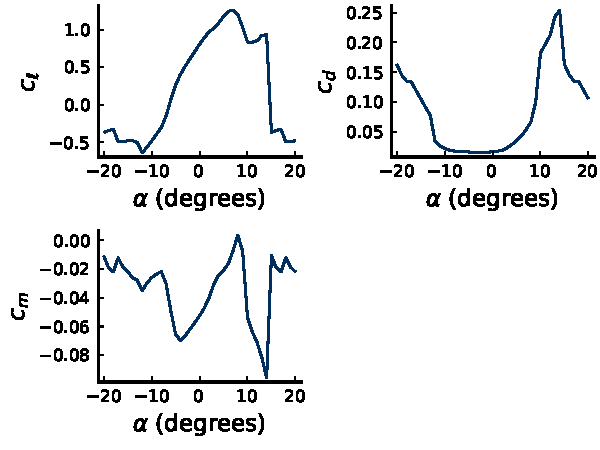
\includegraphics{../graphics/aoa-coefficients.pdf}
		\caption{\emph{The coefficients of lift, drag, and moment plotted against angle of attack for a NACA 2412 airfoil.}}
		\label{fig:aoa-coefficients}
	\end{figure}
	
	The coefficients of lift (\(C_\ell\)) and drag (\(C_d\)) both increase as angle of attack (\(\alpha\)) increases, because as the angle increases, the pressure differential between the top and bottom of the airfoil becomes larger. This also increases coefficient of moment (\(C_m\)). It is also important to note that figure \ref{fig:aoa-coefficients} establishes that lift is negative when \(\alpha\) is less than zero, which makes sense because the pressure differential goes from having greater pressure on the bottom (positive lift) to greater pressure on the top of the airfoil (negative lift). It can also be seen that the zero-lift angle of attack is somewhere between 0 and 0.5 degrees, which is where the lift changes from negative to positive. It appears that stall takes place at an angle of attack of about 10 degrees. This happens when the angle of attack becomes too great and the flow becomes detached, so that the airfoil can no longer produce lift. It can be clearly seen on the lift and drag plots.\\
	
	In order to see the accuracy of Xfoil, the results gained from Xfoil were plotted against experimental data from a study done on the NACA 2412 airfoil (see figure \ref{fig:airfoil-comparison}).\\
	
	\begin{figure}[H]
		\centering
		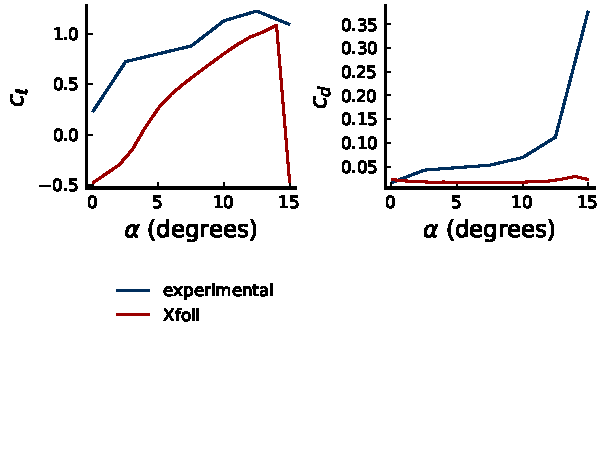
\includegraphics{../graphics/airfoil-compare.pdf}
		\caption{\emph{The comparison of data collected experimentally to data collected from Xfoil.}}
		\label{fig:airfoil-comparison}
	\end{figure}
	
	It is interesting to see that the experimental lift curve looks very similar to the one obtained from Xfoil, except shifted up. Also, the drag curves between experimental and Xfoil are very different. The reason for this is unknown, although it might be an error in Xfoil calculations.\\
	
	Next to be evaluated was how varying the Reynolds number affects the airfoil polar. The purpose of the Reynolds number is to compare inertial forces to viscous forces. A high Reynolds number is an indicator that fluid flow will be turbulent, where as a low Reynolds number is an indicator of laminar flow. In figure \ref{fig:altered-reynolds}, the relationships between Reynolds number and the coefficients are shown.\\
	
	\begin{figure}[H]
		\centering
		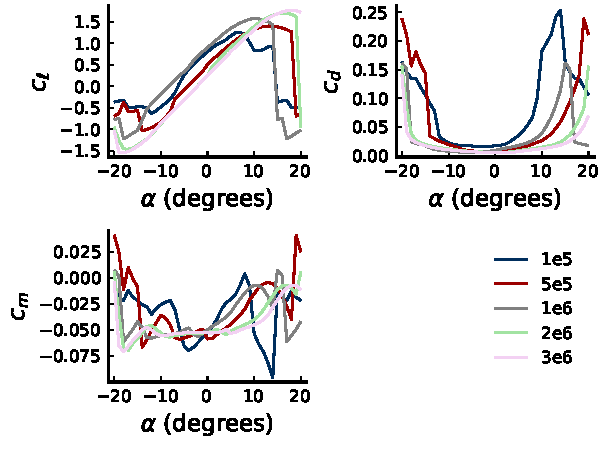
\includegraphics{../graphics/altered-reynolds.pdf}
		\caption{\emph{The lift, drag, and moments against angle of attack for varying Reynolds numbers.}}
		\label{fig:altered-reynolds}
	\end{figure}
	
	As the Reynolds number increases, it seems that all the curves become more smooth. Also, as the Reynolds number increases, the curves of drag and moment become more leveled out. These results make logical sense, because changes in how turbulent the flow is doesn't affect the lift generated as much. On the other hand, higher Reynolds numbers and therefore more turbulent flow decreases the drag and moment at more extreme angles of attack (see figure \ref{fig:altered-reynolds}). The reason for these effects is higher Reynolds numbers means that the fluid flow around the airfoil doesn't have as much of an effect on it. This is also why the curves seem to converge as the Reynolds number increases.\\
	
	As for physical attributes of the airfoil, its thickness and camber were changed to see their effect. The thickness of an airfoil is the greatest distance between the upper and the lower surfaces of an airfoil. In figure \ref{fig:altered-thickness}, the relationship between airfoil thickness and the coefficients of lift, drag, and moment can be seen.\\
	
	\begin{figure}[H]
		\centering
		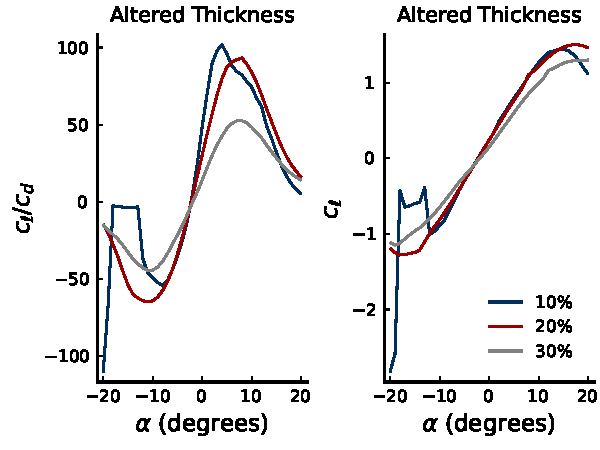
\includegraphics{../graphics/altered-thickness.pdf}
		\caption{\emph{The ratio of lift to drag coefficients and coefficient of lift against angle of attack.}}
		\label{fig:altered-thickness}
	\end{figure}
	
	As the thickness of the airfoil increases, the ratio of lift to drag curve becomes more shallow. This is because increasing thickness leads to lift and drag becoming closer and closer to each other, either because lift is decreasing, drag is increasing, or a combination of the both. It can be seen in the lift vs. angle of attack plot of figure \ref{fig:altered-thickness} that increasing thickness leads to decreasing coefficients of lift for all angles of attack, thus explaining why the lift over drag curves become more leveled out for increased airfoil thickness. Additionally, figure \ref{fig:altered-thickness} displays that the zero lift angle of attack remains the same, but the angle of attack at which stall takes place is increased slightly as airfoil thickness increases.\\
	
	The camber of an airfoil is the measure of the asymmetry between the two acting surfaces of an airfoil. An airfoil with zero camber is symmetric. In figure \ref{fig:altered-camber}, the effect of different cambers can be seen.\\
	
	\begin{figure}[H]
		\centering
		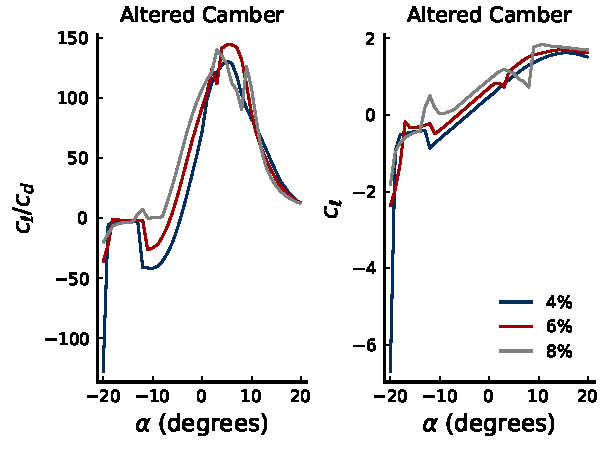
\includegraphics{../graphics/altered-camber.pdf}
		\caption{\emph{The ratio of lift to drag coefficients and coefficient of lift against angle of attack.}}
		\label{fig:altered-camber}
	\end{figure}
	
	As the camber of the airfoil increases, the lift to drag ratio is increased for all angles of attack (see figure \ref{fig:altered-camber}). The reason for this can be seen in the lift coefficient vs. angle of attack plot (see figure \ref{fig:altered-camber}); with increasing camber comes increased coefficients of lift for every angle of attack. Increasing camber leads to an increase in generated lift because more asymmetric shapes lead to greater pressure differentials between the top and bottom surfaces of the airfoil.\\
	
	\subsection{Airframe Analysis}
	
	In order to see the relationship between aspect ratio and the efficiency, the inviscid span efficiency (see equation \ref{eqn:efficiency}) was calculated for airframes with aspect ratios (see equation \ref{eqn:aspect-ratio}) ranging from 3 to 15. After the program calculated the efficiency, it produced a plot shown in figure \ref{fig:efficiency}.\\
	
	\begin{figure}[H]
		\centering
		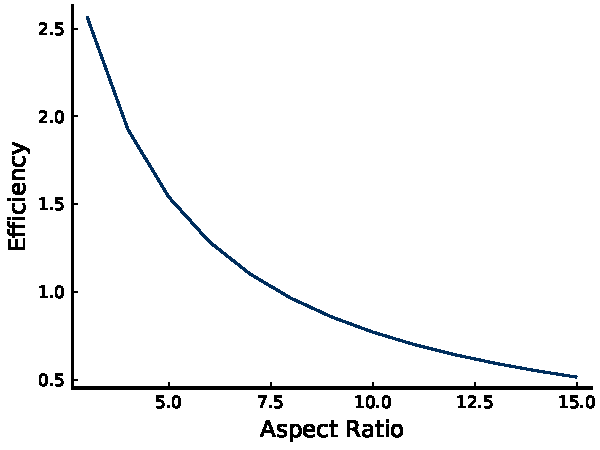
\includegraphics{../graphics/efficiency.pdf}
		\caption{\emph{The relationship between aspect ratio and inviscid span efficiency.}}
		\label{fig:efficiency}
	\end{figure}
	
	In reality, figure \ref{fig:efficiency} doesn't show a relationship that is actually interesting, but it does mathematically plot it correctly. It is simply the definition of inviscid span efficiency.\\
	
	Another characteristic of these airframes that was observed was their stability derivatives. Stability derivatives were calculated for airframes with different tail volume ratios, both vertical and horizontal. The definitions of those ratios are equations \ref{eqn:vtail-ratio} and \ref{eqn:htail-ratio}. Airframes were evaluated with vertical tail volume ratios that varied from 0.001 to 0.0156 and horizontal tail volume ratios that varied from 0.001 to 0.1458.\\ 
	
	In figure \ref{fig:vtail-stability}, we can see that the airframe is stable for vertical tail volume ratios greater than 0.003, but it becomes unstable when the ratio is less than 0.003, at around 0.002. Figure \ref{fig:htail-stability} shows that the airframe is stable for horizontal tail volume ratios greater than 0.05, but becomes unstable when the ratio is less than 0.05, at around 0.025.\\
	
	\begin{figure}[H]
		\centering
		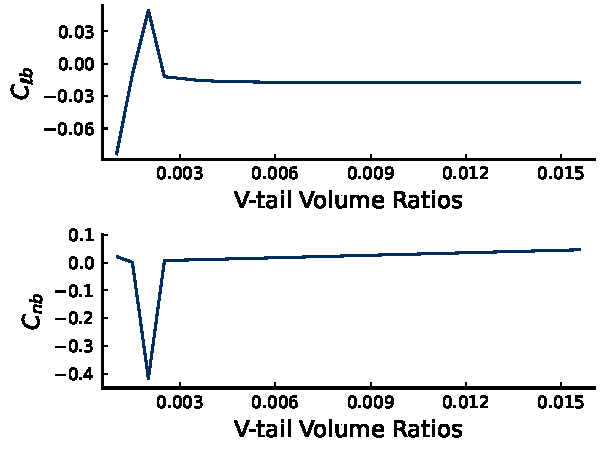
\includegraphics[scale=0.73]{../graphics/vtail-stability.pdf}
		\caption{\emph{This diagram shows the relationship between vertical tail volume ratio, \(C_{\ell{b}}\), and \(C_{nb}\).}}
		\label{fig:vtail-stability}
	\end{figure}
	
	\begin{figure}[H]
		\centering
		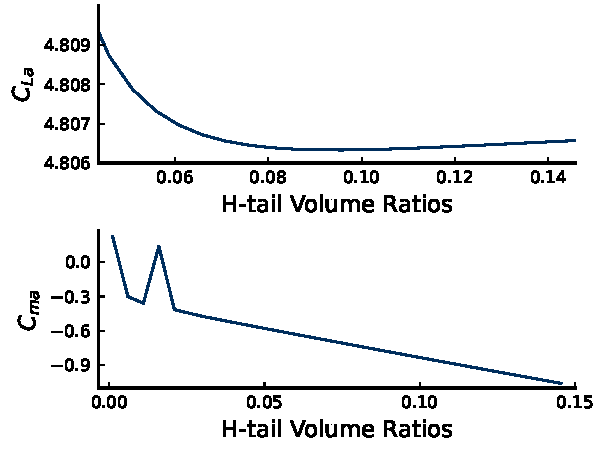
\includegraphics[scale=0.73]{../graphics/htail-stability.pdf}
		\caption{\emph{The relationship between horizontal tail volume ratio, \(C_{La}\), and \(C_{ma}\).}}
		\label{fig:htail-stability}
	\end{figure}
	
	In section \ref{sec:airfoil}, it was found that as angle of attack increases, the lift coefficient also increases, up to a certain point. At that point, the lift coefficient sharply drops, and this is where stall takes place. In that section, Xfoil.jl \cite{McDonnell} was used to calculate the lift coefficient for varying angles of attack. A relationship between angle of attack and lift was also found here, but VortexLattice.jl \cite{McDonnell-Ning} was used instead. A plot was produced showing that relationship (see figure \ref{fig:aoa-lift}).\\
	
	\begin{figure}[H]
		\centering
		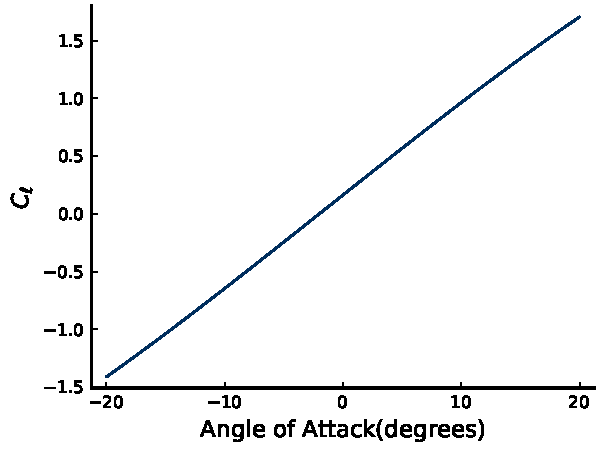
\includegraphics{../graphics/aoa-lift.pdf}
		\caption{\emph{The relationship between angle of attack and lift for an airframe.}}
		\label{fig:aoa-lift}
	\end{figure}
	
	In comparison to the plot created using Xfoil.jl \cite{McDonnell} (see figure \ref{fig:aoa-coefficients}), figure \ref{fig:aoa-lift} looks very similar between angles of attack of -10 and 10. However, past those angles of attack is where it differs. In the Xfoil plot, it shows very clearly where stall would take place, but in this VortexLattice plot, the plot continues linearly and never drops off, never indicating stall. This is why the Vortex Lattice method is not always accurate. It is only accurate when the angle of attack is small, because it assumes that the flow is inviscid at all angles of attack. This is why in figure \ref{fig:aoa-lift} it looks very linear and does not indicate where stall would take place, where as the Xfoil plot does.\\
	
	\subsection{Airframe Design}
	
	After running the program that the optimized the airframe design under the given constraints, it was found that the most optimized airframe was one that had the following characteristics (figure \ref{fig:ideal_design} shows what the design looks like):
	
	\begin{figure}[H]
		\centering
		\caption{\emph{The physical attributes of the optimized airframe design.}}
		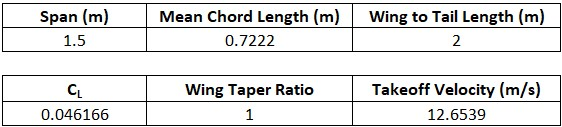
\includegraphics{../graphics/ideal_attributes.jpg}
		\label{fig:ideal_attr}
	\end{figure}
	
	\begin{figure}[H]
		\centering
		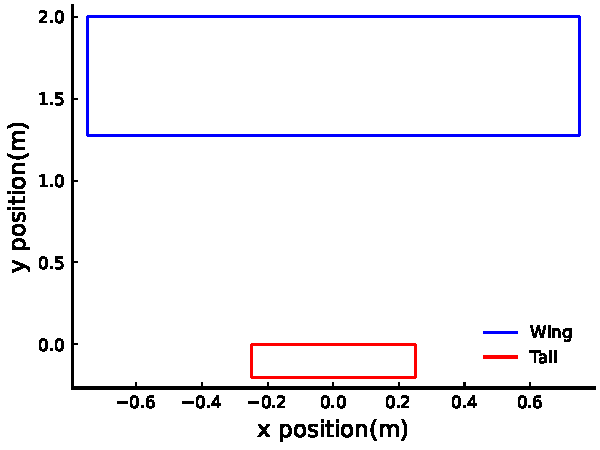
\includegraphics{../graphics/ideal_design.pdf}
		\caption{\emph{The design of the optimized airframe.}}
		\label{fig:ideal_design}
	\end{figure}
	
	The aforementioned necessary lift was 4.905 Newtons. This number was found by multiplying 0.5 kilograms by 9.81 \(m/s^2\), which is the acceleration due to gravity. It is also important to note that the optimization program created for this makes sure that the optimized airframe is also stable. In order to show that this airframe has been optimized, other airframes have been evaluated in order to show correctness.\\
	
	When evaluating an airframe that has a mean chord length that is less than 0.722 m (I used 0.6 m for comparison), it was found that the velocity needed to generate the necessary lift was 13.049 m/s, which is greater than the velocity needed for the optimized airframe. This shows that airframes with smaller mean chord lengths are not more optimized, as they need a greater velocity to lift the 0.5 kilograms.\\
	
	\begin{figure}[H]
		\centering
		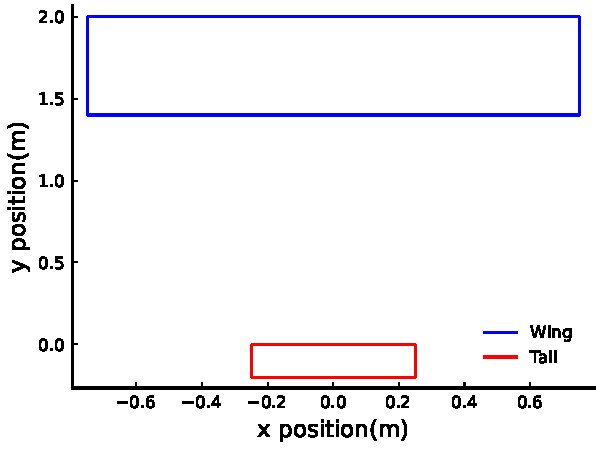
\includegraphics{../graphics/chord_design.pdf}
		\caption{\emph{The design of an airframe with a chord length of 0.6 m.}}
		\label{fig:chord_design}
	\end{figure}
	
	An airframe with a greater chord length was not evaluated for comparison, because of the constraint I put on the aspect ratio. 0.7222 m was the largest possible chord length that kept the aspect ratio of the wing greater than 2.0.\\
	
	Plots showing the lift coefficient vs. angle of attack and drag coefficient vs. angle of attack for these 2 designs are given (see figure \ref{fig:chord_coeff}). They show that the 0.6 m mean chord length design has a lift vs. angle of attack curve that is steeper than the ideal design's. Because of this, it may seem that the alternate design would lead to a smaller takeoff velocity, since it has greater lift coefficients. However, the equation used to calculate takeoff velocity (equation  \ref{eqn:needed-velocity}) uses both the lift coefficient and the reference area. This explains why a larger lift coefficient does not necessarily mean that the takeoff velocity is less. The product of lift coefficient and reference area needs to maximized in order to minimize the takeoff velocity, which is what a mean chord length of 0.722 m does.
	
	\begin{figure}[H]
		\centering
		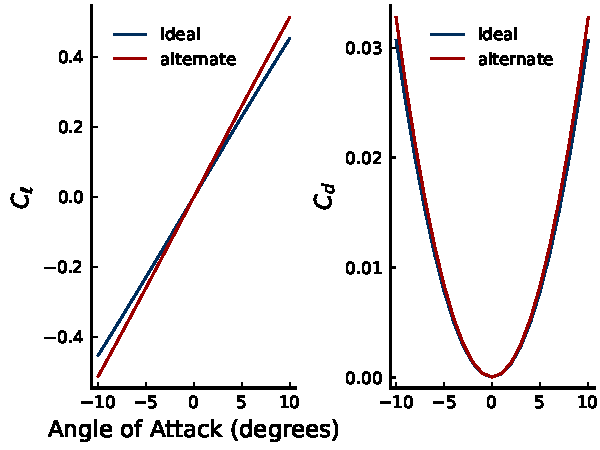
\includegraphics{../graphics/chord_coeff.pdf}
		\caption{\emph{The lift and drag coefficients for varying angles of attack for the 2 designs evaluated using different mean chord lengths.}}
		\label{fig:chord_coeff}
	\end{figure}
	
	When evaluating an airframe that has a length from wing to tail that is less than 2.0 m (I used 1.0 m), it was found that the velocity needed to generate the necessary lift does not change. However, the airframe is less stable as the yaw stability derivative(\(C_{nb}\)) is less than the yaw stability derivative for the optimized airframe. Therefore, as the length from wing to tail is decreased, the airframe becomes less stable. While there are other designs that are still stable with a decreased length from wing to tail, the optimized design's is the upper limit on the constraint put on the length from wing to tail because the optimizing program goes through all the possible lengths, and 2.0 m is the last one it tries.\\
	
	Figures showing the lift and drag coefficients vs. angle of attack for the 2 designs are given (see figure \ref{fig:wingtail_coeff}). They show that the length from wing to tail doesn't affect the lift or drag plots.\\
	
	\begin{figure}[H]
		\centering
		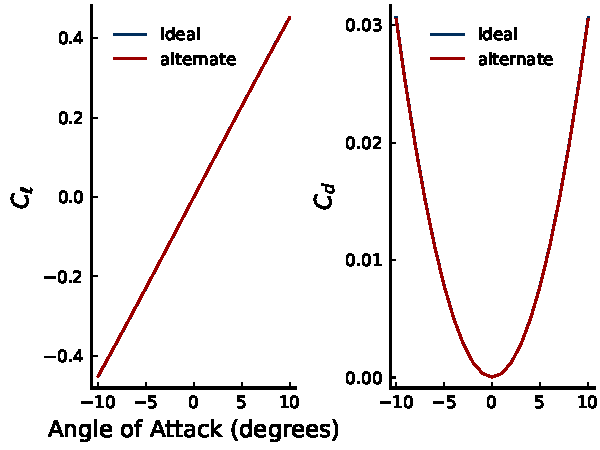
\includegraphics{../graphics/wingtail_coeff.pdf}
		\caption{\emph{The lift and drag coefficient vs. angle of attack for the 2 designs evaluated.}}
		\label{fig:wingtail_coeff}
	\end{figure}
	
	\begin{figure}[H]
		\centering
		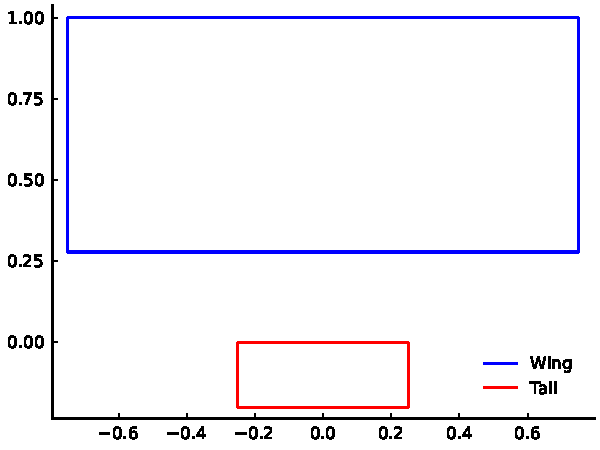
\includegraphics{../graphics/length_design.pdf}
		\caption{\emph{The design of an airframe with a length from wing to tail of 1.0 m.}}
		\label{fig:length_design}
	\end{figure}
	
	The wing taper ratio of an airframe is found using equation \ref{eqn:taper-ratio}.
	
	\begin{equation}
		Taper\ Ratio = \frac{tip\ chord\ length}{base\ chord\ length}
		\label{eqn:taper-ratio}
	\end{equation}
	
	When evaluating an airframe that has a wing taper ratio that is less than 1.0 (I used 0.5), it was found that the velocity needed to calculate the necessary lift was 13.215 m/s. While this is close to the velocity needed for the optimized airframe, it is still larger; therefore, it is not as optimal. This shows that as the wing taper ratio is decreased, the velocity needed to lift 0.5 kilograms increases, making it sub-optimal. You can also see that an airframe with a wing taper ratio of 1.0 has a lift coefficient distribution that is closer to the optimal elliptical distribution than the airframe with a wing taper ratio of 0.5 (see figures \ref{fig:cl_dist} and \ref{fig:cl_dist_compare}).\\
	
	\begin{figure}[H]
		\centering
		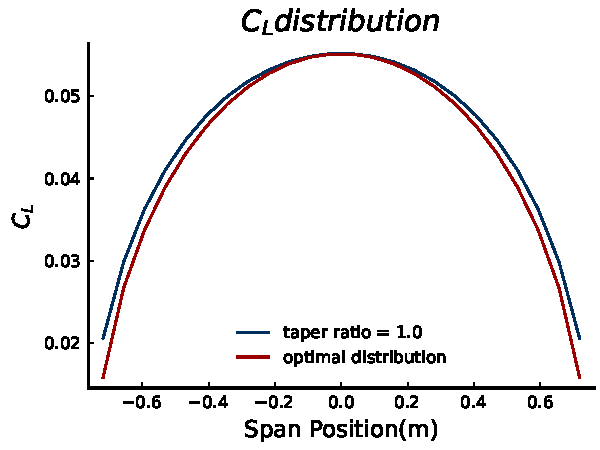
\includegraphics{../graphics/cl_dist.pdf}
		\caption{\emph{The lift coefficient distribution for a taper ratio of 1.0 vs. the optimal elliptical distribution.}}
		\label{fig:cl_dist}
	\end{figure}
	\begin{figure}[H]
		\centering
		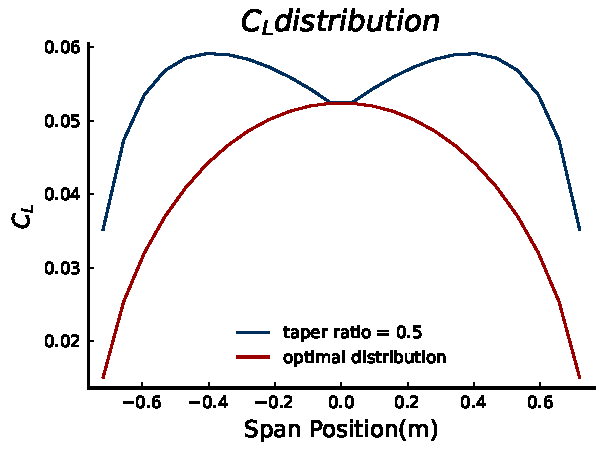
\includegraphics{../graphics/cl_dist_compare.pdf}
		\caption{\emph{The lift coefficient distribution for a taper ratio of 0.5 vs. the optimal elliptical distribution.}}
		\label{fig:cl_dist_compare}
	\end{figure}
	
	Plots showing the lift coefficients and drag coefficients vs. angle of attack for these 2 designs are given (see figure \ref{fig:taper_coeff}). The lift vs. angle of attack plot shows that an airframe with a smaller wing taper ratio has smaller lift coefficients for every angle of attack. However, the reference area remains the same because the mean chord length stays the same. Because the takeoff velocity equation (equation \ref{eqn:needed-velocity}) has the lift coefficient and reference area in its denominator, when only the lift coefficient is decreased, the necessary takeoff velocity is increased. Therefore, designs with smaller wing taper ratios are not as optimal.\\
	
	\begin{figure}[H]
		\centering
		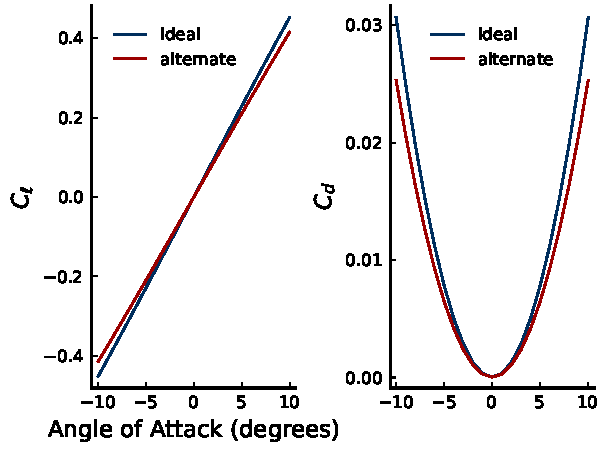
\includegraphics{../graphics/taper_coeff.pdf}
		\caption{\emph{The lift and drag coefficients for varying angles of attack for the 2 designs evaluated using different wing tip tapers}}
		\label{fig:taper_coeff}
	\end{figure}
	
	\begin{figure}[H]
		\centering
		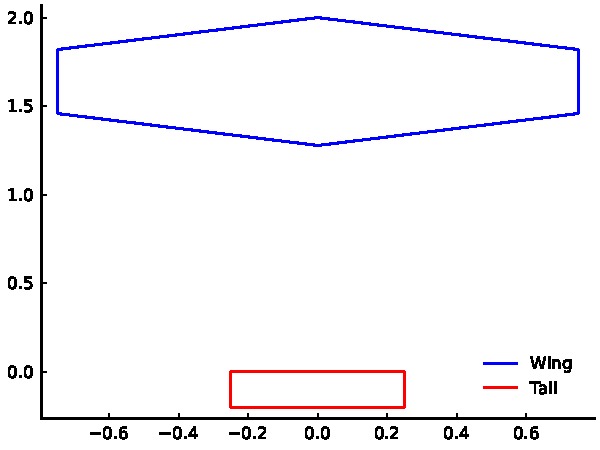
\includegraphics{../graphics/taper_design.pdf}
		\caption{\emph{The design of an airframe with a wing taper ratio of 0.5.}}
		\label{fig:taper_design}
	\end{figure}
	
	
	
	
	
	
	%%%%%%%%%%%%%%%%%%%%%%%%%%%%%%%%%%%%%%%%%%%%%%%%%%%%%%%%%%%%%%%%%%%%%%
	%                                                                    %
	%                            CONCLUSION                              %
	%                                                                    %
	%%%%%%%%%%%%%%%%%%%%%%%%%%%%%%%%%%%%%%%%%%%%%%%%%%%%%%%%%%%%%%%%%%%%%%
	
	\section{Conclusions and Future Work}
	\label{sec:conclusions}
	
	By designing an actual airframe using the skills and knowledge gained from the research done on airfoils and airframes, I learned valuable insights. One of the more important things I learned from optimizing the airframe was that when writing computer programs to solve optimization problems, it is important to make sure that the program accounts for realistic outputs. In the case of optimizing an airframe, I had to put constraints on the aspect ratio so that the mean aerodynamic chord length was a realistic value. If I hadn't done that, the program would have outputted an airframe with the max chord length possible, because mathematically, that is optimal. I also learned that there is a plethora of design variables that can be altered when designing an airframe, which makes it important to only alter a few at a time to be able to see their effects better. From the research on airfoils and airframes, I learned about what effects airfoil polar, how to use tools such as Xfoil.jl \cite{McDonnell} and VortexLattice.jl \cite{McDonnell-Ning} to evaluate airfoils and airframes, and how those tools compare to actual experimental data.\\
	
	From my research, I discovered that as angle of attack increases, the lift of an airfoil and airframe increases. Also, drag vs. angle of attack has a parabolic curve. I also found that increased length from wing to tail of an airframe leads to greater stability. From designing my own airframe, I found that increased mean chord length leads to a greater lift coefficient, but that it does not necessarily mean a lower necessary takeoff velocity. Future work may include building a physical prototype of the airframe I designed, or optimizing my airframe design with a different objective function than the one I used.\\
	
	
	
	
	
	%%%%%%%%%%%%%%%%%%%%%%%%%%%%%%%%%%%%%%%%%%%%%%%%%%%%%%%%%%%%%%%%%%%%%%
	%                                                                    %
	%                           BIBLIOGRAPHY                             %
	%                                                                    %
	%%%%%%%%%%%%%%%%%%%%%%%%%%%%%%%%%%%%%%%%%%%%%%%%%%%%%%%%%%%%%%%%%%%%%%
	
	\bibliography{references}{}
	\bibliographystyle{aiaa}
	
	
	
	
	
	%%%%%%%%%%%%%%%%%%%%%%%%%%%%%%%%%%%%%%%%%%%%%%%%%%%%%%%%%%%%%%%%%%%%%%
	%                                                                    %
	%                             APPEDICES                              %
	%                                                                    %
	%%%%%%%%%%%%%%%%%%%%%%%%%%%%%%%%%%%%%%%%%%%%%%%%%%%%%%%%%%%%%%%%%%%%%%
	
	\appendix
	
	
	
\end{document}